\section{Graphic Matroids}


First, we do not define graphs in completely the same way as in the graph theory class. We used the definition that a graph $G$ is an ordered pair $G = (V, E)$ where $V$ is a finite set (of vertices) and $E$ is a collection of two-element subsets of $V$ (of edges). We will extend the notion of edge to include \textit{loops} and \textit{parallel edges}. For this, we will first illustrate the two notions. Intuitively a loop is an edge going from a vertex to itself, one can also have multiple loops on a single vertex.


For example, in the figure \ref{ilustratinloops}, we have a vertex $a$ with a single loop and vertex $d$ with 3 loops.

\begin{figure}[H]
    \centering
    \subfloat[\centering Loops]{
    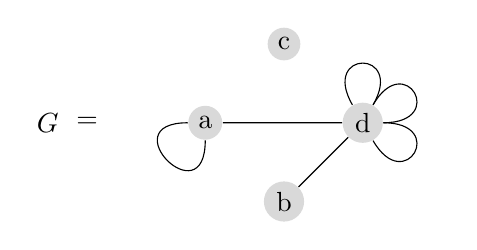
\begin{tikzpicture}[every loop/.style={}]

  \tikzstyle{vertex}=[circle,fill=black!15,minimum size=8pt,inner sep=2pt]

  \node (name) at (-2,0) {$G $};
  \node (another name) at (-1.5,0) {$ =$};
   
  
  \node[vertex] (v2) at (0,0)   {a};
  \node[vertex] (v3) at (1,-1)  {b};
  \node[vertex] (v4) at (1,1)  {c};
  \node[vertex] (v5) at (2,0)  {d};
  \draw (v2) edge[in=270,out=180, loop] node[below] {} ();

  \draw (v5) edge[in=300,out=0, loop] node[below] {} ();
  \draw (v5) edge[in=0,out=60, loop] node[below] {} ();
  \draw (v5) edge[in=60,out=120, loop] node[below] {} ();

  \draw (v2) -- (v5) -- (v3) -- cycle;

  
  %\draw[step=1cm,gray,very thin] (-2,-2) grid (4,4);

%\draw (v1) edge[in=270,out=180, loop] node[below] {2} ();

 
  
\end{tikzpicture}
    
    
    }%
    \qquad
    \subfloat[\centering Parallel edges]{
    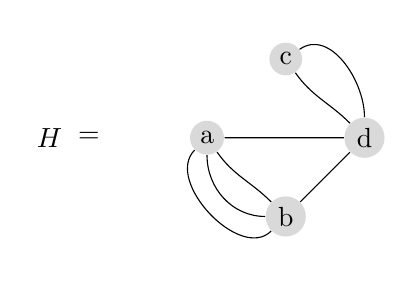
\begin{tikzpicture}[every loop/.style={}]

  \tikzstyle{vertex}=[circle,fill=black!15,minimum size=8pt,inner sep=2pt]

  \node (name) at (-2,0) {$H $};
  \node (another name) at (-1.5,0) {$ =$};
   
  
  \node[vertex] (v2) at (0,0)   {a};
  \node[vertex] (v3) at (1,-1)  {b};
  \node[vertex] (v4) at (1,1)  {c};
  \node[vertex] (v5) at (2,0)  {d};
  
  \draw (v2) edge[in=225,out=225] node[below] {} (v3);
  \draw (v2) edge[in=180,out=270] node[below] {} (v3);
  \draw (v2) edge[in=135,out=305] node[below] {} (v3);

  \draw (v4) edge[in=135,out=305] node[below] {} (v5);
  \draw (v4) edge[in=90,out=35] node[below] {} (v5);


  \draw (v2) -- (v5) -- (v3) -- cycle;

  
  %\draw[step=1cm,gray,very thin] (-2,-2) grid (4,4);

%\draw (v1) edge[in=270,out=180, loop] node[below] {2} ();

 
  
\end{tikzpicture}
    }%
    \caption{Graph $G$ with loops and graph $H$ with parallel edges}%
    \label{ilustratinloops}%
\end{figure}


Above we see graphs $G$ and $H$, one has loops and the other has parallel edges. One way to formalize both constructions, as done in \cite{oxley1} (for them to behave in the way we would like them to behave) is to define a graph to be an ordered pair $(V, E)$, where $V$ is a finite set, so unchanged, however $E$ is a \textit{multiset} of edges. This allows the same two-element subset of $V$ to appear multiple (but at most finitely many) times in $E$, even though it is the same set. Hence, we get parallel edges. For loops, we can get to a multiset consisting of a single element twice, and we also allow it to appear multiple times...
However, the formal construction is not so important, as we will see in the future and one can usually restrict to simple graphs, which are by our terminology the ones without loops or parallel edges. However, we are interested in \textit{properties} loops and parallel edges have. In particular, we see that by our definition of a cycle (a path (a walk (a sequence of adjacent vertices) which does not repeat vertices) which can repeat only one vertex (the ending and the starting vertex)), we have that if a loop is in a cycle, then the whole cycle consists only of that loop - we have one vertex appearing multiple times in a sequence - the beginning/ending vertex. Also, for parallel edges, at most one from a class of parallel edges connecting the same two vertices can appear in a cycle.


\begin{figure}[H]
\centering

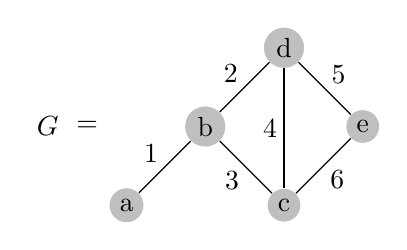
\begin{tikzpicture}[every loop/.style={}]

      \tikzstyle{vertex}=[circle,fill=black!25,minimum size=6pt,inner sep=2pt]

  \node (name) at (-2,0) {$G $};
  \node (another name) at (-1.5,0) {$ =$};
   
  \node[vertex] (v1) at (-1,-1) {a};
  \node[vertex] (v2) at (0,0)   {b};
  \node[vertex] (v3) at (1,-1)  {c};
  \node[vertex] (v4) at (1,1)  {d};
  \node[vertex] (v5) at (2,0)  {e};
  \draw (v1) -- node[midway, xshift=-0.5em, yshift=0.5em]{1} (v2) -- node[midway, xshift=-0.5em, yshift=-0.5em]{3} (v3) -- cycle;
  \draw (v2) -- node[midway, xshift=-0.5em, yshift=0.5em]{2} (v4) -- node[midway, xshift=0.5em, yshift=0.5em]{5} (v5) -- node[midway, xshift=0.5em, yshift=-0.5em]{6} (v3) -- cycle;
  \draw (v4) -- node[midway, xshift=-0.5em, yshift=0em]{4} (v3);

  
  %\draw[step=1cm,gray,very thin] (-2,-2) grid (4,4);

%\draw (v1) edge[in=270,out=180, loop] node[below] {2} ();

 
  
\end{tikzpicture}
\caption{Simple graph on 6 edges}
  \label{simp}

\end{figure}

Consider a concrete example of a simple graph and build a matroid out of it. Let us label the set of edges $E = \{1, 2, 3, \cdots, 6\}$. We will define a collection of subsets $\mathcal{C}$ of $E$ where $C \in \mathcal{C}$ if and only if the set of edges of $C$ forms a cycle in $G$. We check that 

    $$\mathcal{C} = \{\{2,3,4\}, \{4,5,6\}, \{2, 3, 5, 6\}\}.$$

Not surprisingly, the set $E$ with the collection $\mathcal{C}$ being as its set of circuits is, in fact, a matroid, we can check that there is no $\emptyset$ in $\mathcal{C}$, none of its members is properly contained in each other, and finally "circuit elimination axiom" works for all three possibilities of taking pairs of elements of $\mathcal{C}$. We will now prove that this works for a general graph.

\begin{theorem}
Let $G = (V, E)$ be a graph and let $C_1$, $C_2$ be sets of edges of two distinct cycles with a nonempty intersection. Then for any $e \in C_1 \cap C_2$ there exists a cycle $C_3 \subset C_1 \cup C_2 -e$, making the set $E$ of edges into a matroid with the set of circuits equal to the collection of cycles.
\end{theorem}

\begin{proof}

Let the cycle $C_1$ correspond to the sequence of incident vertices  $v_0, \cdots, v_n = v_0$ and let without loss of generality the special edge in the interesection be the edge $e = \{v_0, v_1\}$. Our goal is to find a cycle in the set of edges $C_1 \cup C_2 -e$, which is not difficult, the idea is that we go around $C_1$ until we can jump to $C_2$ for the first time, then we go back to $e$ via $C_2$ from the "backward direction".

Let $k$ be the smallest integer $1<k\leq n$ such that the vertex $v_k$ is in the cycle $C_2$. We know that such an integer exists because $v_n$ is in the cycle $C_2$. 

Let $v_k, w_{k+1}, w_{k+2}, \cdots, v_1$ be the path of vertices in the cycle $C_2$ which does not include the edge $e$. We know that such a path exists, because $C_2$ is a cycle, so from any two distinct vertices, in particular $v_k$ and $v_1$ there are two paths going from $v_k$ to $v_1$ including only the vertices of $C_2$ - we pick the one that does not include the edge $e$.

We claim that the cycle consisting of vertices $v_1, v_2, \cdots v_k, w_{k+1}, \cdots , v_1$ is the desired one and denote its set of edges by $C_3$. By construction the sequence of vertices $v_1, v_2, \cdots v_k, w_{k+1}, \cdots , v_1$ is a cycle, namely the neighboring vertices are incident and except $v_1$ there is no vertex repeating, because we have chosen $v_2, v_3, \cdots v_{k-1}$ to be disjoint from $C_2$. Crucially, $e \notin C_3$ because we have chosen path $v_k, w_{k+1}, \cdots v_1$ to not include the edge $e$ and $v_1, v_2, \cdots v_k$ does not include it because $e = \{v_n = v_0, v_1\}$ and there is no $v_0$ in our cycle. Finally, all of the vertices of $C_3$ are inside the vertices of $C_1$ and $C_2$ by construction so, to conclude the set $C_3$ has the desired property $C_3 \subset (C_1 \cup C_2) - e$.

We have to check to check the possibility that $e$ might be a loop or a parallel edge as well, the above argument works assuming $G$ is a simple graph. If $e$ is a parallel edge than the above argument does still hold since we only now that there is more than one edge between $v_0$
and $v_1$ which does not change anything. However, if $e$ is a loop then by our convention, a cycle consisting of a loop can just be that loop and nothing else, heuristically, because it begins and ends at a single vertex. So $C_1 = C_2 = \{e\}$ which is a contradiction, since we have assumed $C_1$ and $C_2$ are distinct.

To show that the set $E$ is a matroid with the collection $\mathcal{C}$ of cycles as circuits we only have to verify the first two circuit axioms. The empty set is by our defintion not a cycle, because by our defintion a cycle always includes a nonempty set of vertices it is build upon. If there are at least two vertices, than we have incident edges inside, and the only cycle on one vertex is a loop, which is still an edge.

The show the first property suppose we have two sets of edges of cycles such that $C_1 \subset C_2$ and assume for contradiction there is some $e \in C_2 - C_1$. Then (we are assuming neither of the cycles are loops, that case is obvious) the set of edges $C_2 - e$ corresponds to a path from the vertices which $e$ connects. However there is a cycle $C_1 \subset C_2 -e$ which is a subset of a path - a contradiction. So if $C_1 \subset C_2$ then $C_2 - C_1$ is empty, in particular then $C_2 = C1$ and all three circuit axioms are satisfied.



\end{proof}

\begin{defn}
    We call a matroid $M$ graphic if it is isomporphic to $(E, \mathcal{I})$ where $E$ is the set of edges of some graph and the set of circuits is given by the set of all edge cycles.
\end{defn}

We thus know that given any graph $G$ we have natural matroid structure on its set of edges, by declaring graph cycles to be circuits. Because we know other equivalent descriptions of matroids it is natural to ask what are the independent sets or bases in the case of graphic matroids. 

Suppose that the set of edges $B$ is a base of a graphic matroid. We know that this means that $B$ is independent (interpretation of which in the case of graphic matroids we do not yet know) however, adding any element of $E-B$ to $B$, i.e. any edge not in $B$ to $B$, we get a \textit{dependent set}, which means it contains a circuit. By our defintion this means that it has to contain an edge cycle. Combining all we see that the set of edges $B$ has the property that it does not contain any cycles, however adding any edge makes a cycle - this is the precisely one of the equivalent characterizations of \textit{spanning forrests} - we cannot say spanning trees because the graph might not be connencted. 

Any independent set is a subset of some basis, so in graphic matroids the set of edges that is independent has to be a subset of some spanning forrest, which means it is just a forrest.

As an example we will show that many matroids shown until now are, in fact, graphic. 


 
\begin{figure}[H]
    \centering
    \subfloat[\centering Matrix $A$]{

    $$A = \begin{pmatrix}
        
        2 & 0 & 2 & 0 \\
        1 & -1 & 0 & 0 \\
        0 & 3 & 3 & 0
        
        
        \end{pmatrix}$$
        
    
    
    }
    \qquad
    \subfloat[\centering Graph $H$]{
    \begin{tikzpicture}[every loop/.style={}]

  \tikzstyle{vertex}=[circle,fill=black!15,minimum size=8pt,inner sep=2pt]

  \node (name) at (-2,-1.5) {$H $};
  \node (another name) at (-1.5,-1.5) {$ =$};
   
  
  \node[vertex] (v2) at (-1,-2)   {};
  \node[vertex] (v3) at (1,-2)  {};
 
  \node[vertex] (v5) at (0,-1)  {};
  

  \draw (v2) -- node[midway, xshift=0em, yshift=-0.5em]{1} (v3)  -- node[midway, xshift=0.6em, yshift=em]{2} (v5) -- node[midway, xshift=-0.6em, yshift=0em]{3} (v2)  --cycle;
  
  \draw (v5) edge[in=150,out=30, loop] node[above] {4} ();
  
  %\draw[step=1cm,gray,very thin] (-2,-2) grid (4,4);

%\draw (v1) edge[in=270,out=180, loop] node[below] {2} ();

 
  
\end{tikzpicture}
    }%
    \caption{Matroid $M[A]$ is graphic; it is isomprphic to the graphic matroid $G$}%
    \label{graphic}%
\end{figure}

In \ref{graphic} we see that the graph $H$ exactly to corresponds to the vector matroid formed on matrix $A$. Edge 4 is a loop, so a dependent set, corresponding to the fact that the fourth column is a zero vector. Similarly, any two element sets of nonzero vector are independent, corresponding to the fact that any two non-loop edges do not form a cycle in the graph. Finally, any set of three or more edges in dependent, which is easily seen in the graph because we have 3 vertices so the size of a spanning forrest is at most 3 - 1 = 2.


